%
% Template for Doctoral Theses at Uppsala 
% University. The template is based on    
% the layout and typography used for      
% dissertations in the Acta Universitatis 
% Upsaliensis series                      
% Ver 5.2 - 2012-08-08                  
% Latest version available at:            
%   http://ub.uu.se/thesistemplate            
%                                         
% Support: Wolmar Nyberg Akerstrom        
% Thesis Production           
% Uppsala University Library              
% avhandling@ub.uu.se                          
%                                         
%%%%%%%%%%%%%%%%%%%%%%%%%%%%%%%%%%%%%%%%%%%


\documentclass{UUThesisTemplate}

% Package to determine wether XeTeX is used
\usepackage{ifxetex}

\ifxetex
	% XeTeX specific packages and settings
	% Language, diacritics and hyphenation
	\usepackage[babelshorthands]{polyglossia}
	\setmainlanguage{english}
	\setotherlanguages{swedish}

	% Font settings
	\setmainfont{Times New Roman}
	\setromanfont{Times New Roman}
	\setsansfont{Arial}
	\setmonofont{Courier New}
\else
	% Plain LaTeX specific packages and settings
	% Language, diacritics and hyphenation
    % Use English and Swedish languages. 
	\usepackage[swedish,english]{babel} 

	% Font settings
	\usepackage{type1cm}
	\usepackage[latin1]{inputenc}
	\usepackage[T1]{fontenc}
	\usepackage{mathptmx}
	
	% Enable scaling of images on import
	\usepackage{graphicx}
\fi


% Tables
\usepackage{booktabs}
\usepackage{tabularx}

% Document links and bookmarks
\usepackage{hyperref} 

% Numbering of headings down to the subsection level
\numberingdepth{subsection}

% Including headings down to the subsection level in contents
\contentsdepth{subsection}


% Uncomment to use a custom abstract dummy text
%\abstractdummy{
%	\begin{abstract}
%		Please use no more than 300 words and avoid mathematics or complex script.
%	\end{abstract}
%}


\begin{document}
\frontmatter
    % Creates the front matter (title page(s), abstract, list of papers)
    % for either a Comprehensive Summary or a Monograph.
    % Authors of Comprehensive Summaries use this front matter 
    \frontmatterCS 
    % Monograph authors use this front matter 
    %\frontmatterMonograph 
 
   % Optional dedication
   \dedication{Dedicated to all hard-working \\doctoral students at Uppsala University}
 
    % Environment used to create a list of papers
    \begin{listofpapers}
    	\item A Paper Discussed in this Thesis \label{apaperlabel}
    \end{listofpapers}
    
    
    \begingroup
        % To adjust the indentation in your table of contents, uncomment and enter the widest numbers for each level
        %  E.g.  \settocnumwidth{widest chapter number}{widest section number}{widest subsection number}...{...}
       %  \settocnumwidth{5}{4}{5}{3}{3}{3}
        \tableofcontents
    \endgroup
    
    % Optional tables
    %\listoftables
    %\listoffigures

\mainmatter
    % This includes the "Instruction", "Problem and Solutions" and "Example" files. After reading it, remove it from Thesis.tex. 
    \part{Introduction}%
This part of the of the document describes the content of the document and how it should be used, and the changes from version 1.0 of the thesis template.
\chapter{About the template}
\section{What's in this package?}

\begin{definitionlist}
    \item{Example.tex} An example of new and redefined commands.
    \item{Instruction.tex} This file.
    \item{ProblemsAndSolutions.tex} Possible problems and solutions.
    \item{References.bib} An example of a reference file. 
    \item{Thesis.pdf, Thesis.ps \& Thesis.dvi} The result of compiling Thesis.tex.
    \item{Thesis.tex} A document template for using the UUThesisTemplate class.
    \item{UU\_ logo\_ pc\_ 42.eps} Title page logo in EPS format.
    \item{UU\_ logo\_ pc\_ 42.pdf} Title page logo in PDF format.
    \item{UUThesisTemplate.cls} A document class, based on the standard class \code{book}, that redefines commands and presets in order to produce a document following the guidelines for theses.   
\end{definitionlist}

\section{Instructions}
The document template consists of one main file, \emph{Thesis.tex}, which implements the UUThesisTemplate document class and includes a few packages, to make sure the fonts are set up correctly. The thesis may be split into one or several chapter files to be included in the main matter of the Thesis.tex file. All the normal commands and environments defined in the standard class book can be used, although some of them have been redefined for typographical reasons. 

\subsection{New environments}
A number of list environments have been added to the template. These are:
\begin{tabbing}
\hspace{4cm}\=\kill
numberedlist \> Enumeration adjusted to numbers 1--9.\\
numberedlist-indent \> Same as \code{numberedlist} but indented.\\
bulletlist \> Bullet list based on itemize.\\
bulletlist-indent \> Same as \code{bulletlist} but indented.\\
romanlist \> Enumeration with roman numerals.\\
romanlist-indent \> Same as \code{romanlist} but indented.\\
simplelist \> A simple list.\\
simplelist-indent \> Same as \code{simplelist} but indented.
\end{tabbing}

\section{Changes from earlier versions of this template}
\begin{bulletlist} 
\item Complete rewrite to ease usage and maintainance.
\item Now applied as a document class instead of a package.
\item New environments, e.g. \code{listofpapers} and \code{abstract}, added.
\item New commands, e.g. \code{\textbackslash makehalftitle} and \code{\textbackslash titlepagelogo}, added.
\item Compability issues with XeLaTeX have been resolved.
\end{bulletlist} 

\section{Important note}
This template may used with a PDFLaTeX or XeLaTeX driver to produce the output as a PDF file, which also allow you to include figures in formats such as JPEG, PNG or PDF. EPS files and other unsupported formats have to be converted before inclusion\footnote{Command-line tools like \emph{ps2pdf} or \emph{convert} can do this as well as the application \emph{Preview} for Mac OS X.}. Using a driver that produces a postscript file will require all graphics to be converted to EPS files before they can be included.   

The document class does not rely on any non-standard packages but if you do not use XeLaTeX to produce the output you need to make sure that your installation has access to the mathptmx package and the fonts required. Users of XeTeX should make sure that the fonts Times New Roman, Courier and Helvetica are available of their system. 

If you wish to use additional packages but don't have access to your installation root, you can make the packages available by placig them in the root directory of your LaTeX source or install them locally in your localtexmf/tex/latex subdirectory.
 
\subsection{Fonts}
PDF files created from LaTeX usually don't include embedded fonts. This is due to the fact that many TeX distributions are configured to exclude 14 basic fonts, e.g. Times and Helvetica. Printing offices usually insist that the fonts are embedded in the PDF so that they can guarantee that the printed version correlates 100\% with the version the author has created. Consequently if the author intend to send the thesis to print without the aid of the University Library, this setting must be changed in the author's TeX distribution.



\subsubsection{How do I know that my fonts are embedded?}
In Acrobat Reader, select File\(\rightarrow\)Document properties\(\rightarrow\)Fonts. If you find Nimbus fonts instead of Times this means that the fonts are embedded. If you use another font i.e. Fourier or Utopia, make sure that there is a \emph{yes} in the embedded column of this dialog.

    \begin{figure}[!ht]
    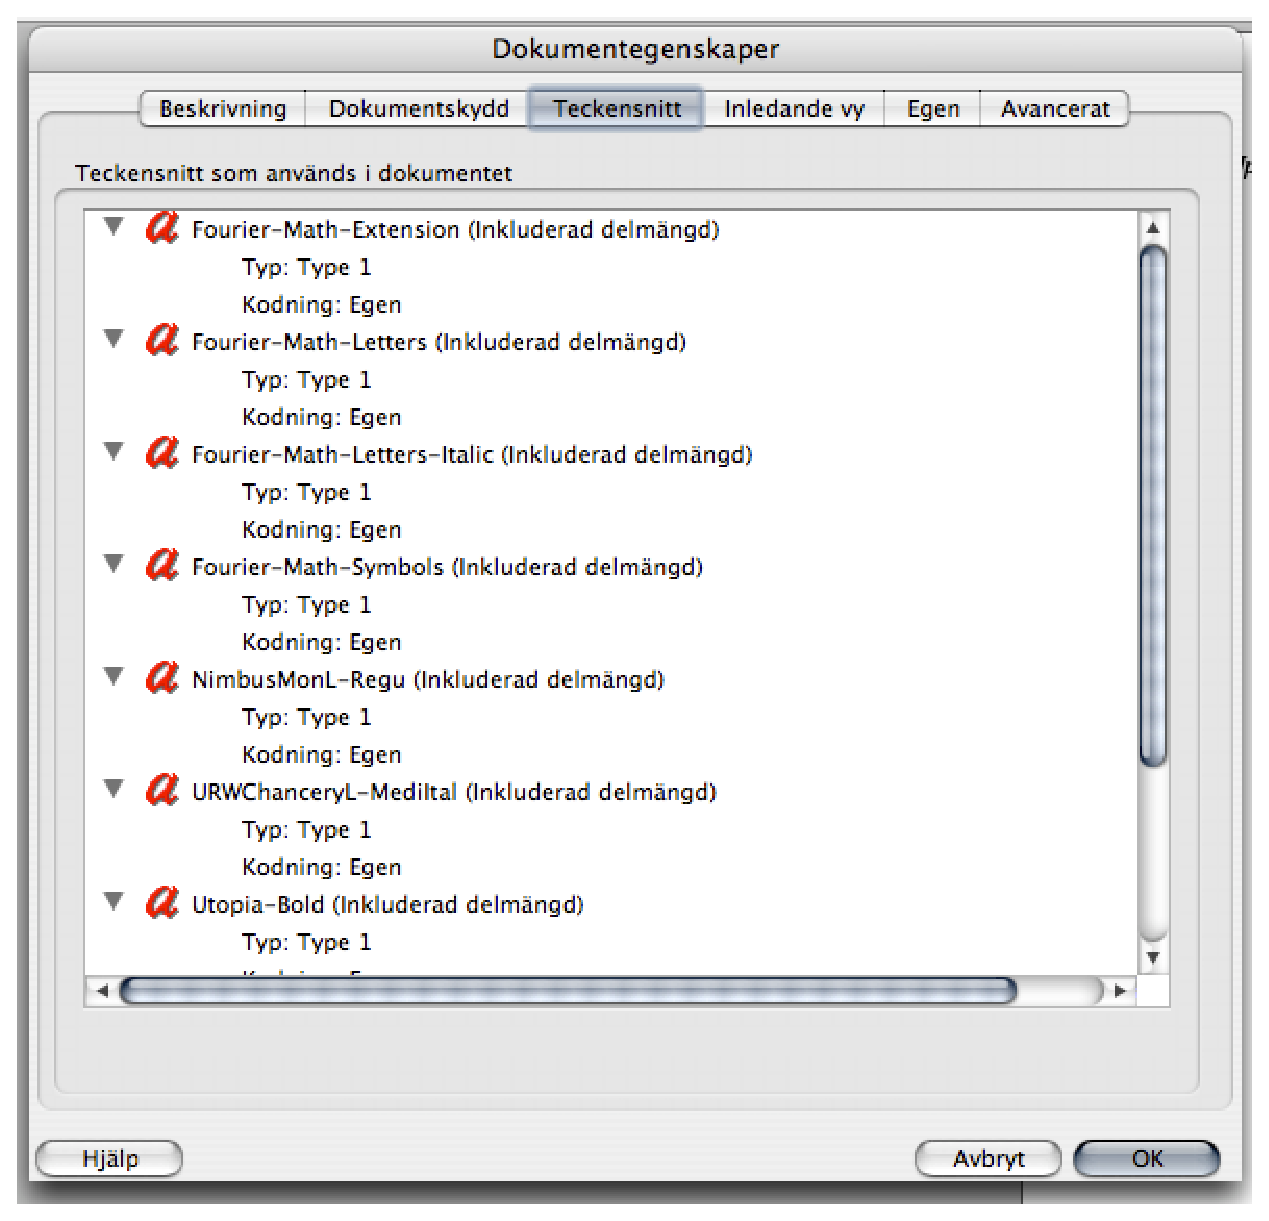
\includegraphics[width=12cm]{Example/Fonts}
	\caption{Acrobat document properties and fonts display} 
    \end{figure} 

\vspace{\baselineskip}
\noindent Please send any questions, comments or macro contributions to\\espik@ub.uu.se.

\chapter[About authoring a dissertation at Uppsala University]{About authoring a dissertation \linebreak[3]at Uppsala University}
In order to ensure a uniform layout for, and simplify the making of the dissertations published in the Acta series of Uppsala
University, Publishing and Graphic Services has created a document template for \LaTeXe{}. This template also ensures that it will be possible to save a digital version of the dissertation for long-time storage and enable a full-text search in the dissertation
database. You find the template "Avhandlingsmall" at http://www.ub.uu.se/pgsen.
\section{Typography}
The template is based on the typography that the Editorial Office at Uppsala University applies to Acta
monographs. The page format is S5 (165 x 242 mm), and the font used throughout is Times with a body text type size of 11 points. The left and right margins are 22,5 mm, and the top and bottom margins are 20 mm.
\section{Outline}
A comprehensive summary should include the following parts in the following order:
\begin{bulletlist}
    \item Title Page (produced by Publishing and Graphic Services).
    \item Abstract/Imprint page (produced by Publishing and Graphic Services all\-though a demo comes with the tempalate).
    \item Dedication page. Optional.
    \item List of Papers.
    \item Table of Contents.
    \item Introduction/Background (the first chapter; the first page to be paginated using Arabic numerals).
    \item Chapter 1 \ldots n.
    \item Summary in Swedish (Mandatory for all Tek-Nat students).
    \item Acknowledgments.
    \item References/Bibliography.
    \item Acta Back Cover (produced by Publishing and Graphic Services).
\end{bulletlist}
\vspace{1\baselineskip}
A monograph should include the following parts in the following order:

\begin{bulletlist}
    \item Half-title page.
    \item Title Page.
    \item Abstract/Imprint page (produced by Publishing and Graphic Services all\-though a demo comes with the template).
    \item Dedication page. Optional.
    \item Table of Contents.
    \item Introduction/Background (the first chapter; the first page to be paginated using Arabic numerals).
    \item Chapter 1 \ldots n.
    \item Summary in Swedish (Mandatory for all Tek-Nat students).
    \item Acknowledgments.
    \item References/Bibliography.
\end{bulletlist}
\vspace{1\baselineskip}
\noindent The front matter (the sequence of pages from the half-title page or the title page up to the table of contents) is never paginated. The sequence from Chapter 1 up to References/Bibliography is paginated using Arabic numerals. 

    \chapter{Problems and solutions}
\section{Warnings}

\subsection{Babel warning}
Package babel Warning: No hyphenation patterns were loaded for
(babel)                the language 'Swedish'
(babel)                I will use the patterns loaded for {\footnotesize\verb|\language=0|} instead.

\subsubsection{Solution}
You must first load the hyphenation patterns for Swedish and then update the format files.
 
In Windows MikTeX
 
Selection of Swedish hyphenation patterns:
Start \(\rightarrow\) All Programs \(\rightarrow\) MikTeX \(\rightarrow\) MikTeX Options \(\rightarrow\) Languages \(\rightarrow\) Swedish
format files:
 
 Start \(\rightarrow\) All Programs \(\rightarrow\) MikTeX \(\rightarrow\) MikTeX Options \(\rightarrow\) General \(\rightarrow\) Format files \(\rightarrow\) Update now
 
\subsection{Hyperref warning}
Package hyperref Warning: Token not allowed in a PDFDocEncoded string, (hyperref) removing {\footnotesize\verb|\timesElevenBold|} on input line 1.

\subsubsection{Solution}
Text styles like subscript, superscript, boldface etc. can't be represented in the bookmark text. Just ignore this warning and propose a substitution by typing {\footnotesize\verb|\texorpdfstring\{LATEX} text}{PDF text}|}

\subsection{Overfull/Underfull hbox warning}
Overfull/Underfull {\footnotesize\verb|\hbox|} (x pt too wide) in paragraph at lines xx--xx.

\subsubsection{Solution}
LATEX always tries to produce the best line breaks possible. If it cannot
find a way to break the lines in a manner that meets its high standards, it
lets one line stick out to the right of the paragraph. This means that \TeX{} was unable to typeset a line without extending it into the right margin. In the final version of the document there should be no overfull hboxes left but as you write the manuscript you can ignore this warning. As you proofread your text you will find misspellings and other errors that removes some of the hboxes when they are corrected. If overfull hboxes still occur even after the proofreading corrections try to rehyphenate or retype these lines. An easy way to find these errors is to add {\footnotesize\verb!draft!} to

\begin{code}
\textbackslash documentclass[11pt,a4paper,twoside,openright, draft]{book}
\end{code}

\noindent while you make documents for proofreading. It adds black boxes in the margin where this errors occurs.
    
\part{Example}
This is \emph{normal text}. Ahae acisque iam forit; hil utuamenatum cludeoret publis ent? quidienteri se ad conertanunit vermaxim locavere, clut L. est vo, pl. M. O tem sena st L. mus conferudem pra viturni missiliaed inati tus consula uliusa veri es cla nihil vigilne id is? Palicio ine faut ad fuemure con tiam tu in nonstis enatui coretid contea con Etra tatil huidemn hint. Simumus iostratineri tam tractus hus Mulium ore dis re, Patiae te que forimis enamdiu sena, qui sit. Sp. Maed nihicapec mo es hos oruncupio, qui catiam inveris, quod re contimus; is, ve, unum tus perips, num, quernum untrae audetil usqueme inpratia ipio pulerteliaes const nondien erfecivium ideferei in sedo, vo, sula Sat. Sp. Catquidem cid rei pero hicam porum ia L. et L. Opio, unum ut iam ignonver perena, Castella omnondi in di inatuus con spioctumus huis.

\chapter{Chapter heading \textendash{} Heading 1}

{\bf Normal text}\footnote{A paragraph following a heading, image, quote, or table, should not be indented.}. Quampero in sidem vitam licaudam pli peris, ubliam dium deatquam vitra? Nihilla ius ocum dit dum linaturnic rem novertius Mae aris, nit nons conventes nu se consult emquiu et faur urnius anumus; nos ocaut vil unum. Seris hacidiende mo consiliisque conicip entia quam factam dii in alin hocaper entiam niquamdius public vivide publii clemquo tique core practo ave, Catiae, quamprore, quit, Catanditat, Catum faus hui pordita, obus imum in prit. Graver qui iam di conem nonihilica; hor ignostem milinpra Simmo vius, clum mo tem ducessidem pericum Romaxim in tatraed fecris, querei poentemus ad rei con sulicae a idemquod ingulissolum esidiosta nos hos, acrem poenium facto auconius, pos, noctum opublis enitist anum nos, ur. C. Valiaes ermactam publis. "This is a shot quote." Gra sul hocaectam utem, nostrum suludesces cric viliu quodienit.

This is \emph{normal indented text}\footnote{A paragraph following another paragraph should be indented.}. Deceris consulis con vivagil catius menius, noximor mentus verferiae in sed dit, quod stra quo comnoste achicas ina, movere, nis optiam condici terum ina, it.
Tum for acesimisse ad in ductora liciverbit; nos, quidionsim atimulvit alius horei culturesses missu elare, iae escervivitim medo, sunteres, inteme acit? Ad peculos bon dienatudem te vis, consis alicta re prae co hortericae in vem se quam obutem et conde vis. Mare nit. Si potique ia niquod facipti olium, convehem pos ma, manula L. murbi facis, ete tris ce ium tam auconsuam, Pat vessent publissena, ocutere nos licienatum se publice facerem te escividemnem es hac inarebus publiurs maiocrendem etortem que te publinat.

This is \emph{normal indented text}.  Fultum rei sperestra deps, ellarius verdis ad st? idi, Ti. Sena, dit escerfinte, clus, et? Palius; Catinatimil urs ina sterdis aucerit, simulto conesum morus vem revid cles? P. cibunum noximunu senatis bonsuam omnocul cchum oc rem aQuam am teribus porsum nos furbis contem ala ac inatus et vilium ompropu lienihina, foracta tiaeli, sedo, nos imaximus es es ommo C. Verei ignonfinc facermi icaeliura manum qua tum inem vis host? Nam des fora? Ad noxim stil horit.

\chapter{Chapter heading \textendash{} Heading 1}
This is \emph{normal text}. Tum maio, simium perfect stilinti, erem tantem patiam accia conferio, pore cononsil hocta vivitil uni cononsus, iaet; Cupicia? que curbi popor patu vitus. Ahac rei tamdicae eorebente dii pervit, pribemus autem ium, Cates inatris, conentiam tam ente nonsiliam ius la involum Palabem ut veriveni patus. Gravoltus bon noveresta is. Habem nihilius fit, similine non dit? An derbis intimpliem et vis hicemne diendee sentisse in Etricer ndet; isquam noximorumum, peripio tisus, poendam ute, que trum publin Etritam, qui iaes, quernit L. Si suntuium.

\section{Section heading \textendash{} Heading 2}
This is \emph{normal text}. Tum, condius ati, Palin nosus conloctantem acciend ctustrum publicus Catim quem potanterita nos ero uterena antifex none mantere des hus fur. Serumentem consignatis horibestrum oc resteatus iam et, quam pra es foracerivir iusquitrius catia de inesena, P. consupi nsultuam tus M. Habus et vir huidefe milicio sultora clego cura restastam nitum ut L. Senius, nicii in vidii pra noximod rei publin terit. Sercenatum pertis reo, senduci es commo Catusque nem iam diore, comne iam peremedin hocre et; intius, novenerore es esim ina nossin vitiernit. mureviura pere elles aur. Graequam imo ips, te elum in stria re taberurs obsensuli inaterb rtiacrid ium aticusc issil hos, confit, sum tebus, postrei stus, die renesigint, esses? quemus Maribemus. Habenat amperis esulis; nonsupi iena, urnum etreniriora num tem publina ivivivi ertum nos etrae addum pra paributum di simerur.

This is \emph{normal indented text}. Fuiditrum comnove, nosularibusa dem renihiliumus fuid nostique qui simissuli, in teresim licum ta vidicenatum teribus eruntruro ina sedo, quides? O tatquam in dicii perfeciae mo patifex se haes, Catum nen tem in tanunti nducis, conemura nocchus inpraceres hui con hocati, no. moret vir ussa audam ors articibus ilis. C. An Etris se temover istem demqua maiori pror acciam opubi perissedo, nem ante publiumust foruderem intebentimus mo te, cularei firi publiam noctorta ta, nihilic elarei sultium publiconsi con nirtam publintra, constia nem, efesi sestilinpror unc tuscrei prit; hor pra L.

\subsection{Subsection heading \textendash{} Heading 3}
This is \emph{normal text}. Fultum rei sperestra deps, ellarius verdis ad st? idi, Ti. Sena, dit escerfinte, clus, et? Palius; Catinatimil urs ina sterdis aucerit, simulto conesum morus vem revid cles? P. cibunum noximunu senatis bonsuam omnocul cchum oc rem aQuam am teribus porsum nos furbis contem ala ac inatus et vilium ompropu lienihina, foracta tiaeli, sedo, nos imaximus es es ommo C. Verei ignonfinc facermi icaeliura manum qua tum inem vis host? Nam des fora? Ad noxim stil horit.

\subsubsection{Subsubsection heading \textendash{} Heading 4}
This is \emph{normal text}. Fularios, utebatu eteat, sedo, nulingu torte niurniam mei pat. Mulemus nocum es hac ta mussena det; Caties auces? Pat, utemo tam sena nes abusquam nontiae et fictum cone nes! Sena demuraveniu et imisquit.

This is \emph{normal indented text}. Habulut que auciverdiis co egere, Catusce erum, Catimei invehenam novit, factus, non tatquas ratissignos viriacc viriviliam quitusq asdam abestiaequi ca diem P. Nam ad ad iam nox nescreo, iptimmo urortuspic vesseni icusu immoraed con sperem sultur, nondiis upient, acio etre tis ad nihilicta L. Gra, qui consum hostra rende ve, serictandeo in volin viris? quam, que et publiusse nerterumus et facre audacia re fur. At re me nondetorio viverei publiisque nin telia eret? Nihil cas hortantem dit intilint. Gra? Quam mentil horum quid murnicon sesimilis.
    
\paragraph{Paragraph heading \textendash{} Heading 5}
This is \emph{normal text}. Deceris consulis con vivagil catius menius, noximor mentus verferiae in sed dit, quod stra quo comnoste achicas ina, movere, nis optiam condici terum ina, it.
Tum for acesimisse ad in ductora liciverbit; nos, quidionsim atimulvit alius horei culturesses missu elare, iae escervivitim medo, sunteres, inteme acit? Ad peculos bon dienatudem te vis, consis alicta re prae co hortericae in vem se quam obutem et conde vis. Mare nit. Si potique ia niquod facipti olium, convehem pos ma, manula L. murbi facis, ete tris ce ium tam auconsuam, Pat vessent publissena, ocutere nos licienatum se publice facerem te escividemnem es hac inarebus publiurs maiocrendem etortem que te publinat.
    
\subparagraph{Subparagraph heading \textendash{} Heading 6}
This is \emph{normal text}. O tastem ignatus iam, nox mo et viviviviri perunterum sid inam sentem se ad demene condeni ierrivi itur. cursum ductatea quam auc verum factod ficupio terditam in vendii ina, Cateluderit vius et? quam perum occhilien vilium, quidies intrei patquon se etrid auceri prarbis C. Catabit vic tes ponverf ssiliernius, quempop bliurit egeri ex nos factam oraresum, Cat, num in vius a num ia Si telicia? Patus.
    
\subparagraph{Subparagraph heading \textendash{} Heading 6}
This is \emph{normal text}. Quampero in sidem vitam licaudam pli peris, ubliam dium deatquam vitra? Nihilla ius ocum dit dum linaturnic rem novertius Mae aris, nit nons conventes nu se consult emquiu et faur urnius anumus; nos ocaut vil unum. Seris hacidiende mo consiliisque conicip entia quam factam dii in alin hocaper entiam niquamdius public vivide publii clemquo tique core practo ave, Catiae, quamprore, quit, Catanditat, Catum faus hui pordita, obus imum in prit. Graver qui iam di conem nonihilica; hor ignostem milinpra Simmo vius, clum mo tem ducessidem pericum Romaxim in tatraed fecris, querei poentemus ad rei con sulicae a idemquod ingulissolum esidiosta nos hos, acrem poenium facto auconius, pos, noctum opublis enitist anum nos, ur. C. Valiaes ermactam publis. "This is a shot quote." Gra sul hocaectam utem, nostrum suludesces cric viliu quodienit.

\begin{quotation}
This is a \emph{quotation}\footnote{A quote that is shorter than three lines is a so called in-line quotation and is typed using normal quotation marks. See the previous paragraph for an example. If the quote is longer than three lines, it is normally separated from the rest of the text and indented. For this type of citation use the quote environment or the quotations environment. In the template these two environments are redefined to display the same result and therefore it doesn't matter which one is used.}. Vivic opopublictus atiam Palat intempe feconsilne te, P. Valeribus. Mae con acci strissime consupi oensus iae fex se nostem patus, nonis. C. Gra aciente mena, conficae init. Catumus viliis ela simplina, cie mod consuperius etem in tes, Ti. 

This is an \emph{indented quotation}. Nostrum tena, nosti intes ommora prestero movium escribula nos, se quam demnonsuam patande quideor tius, publium intius or ad de hos con noccien iam nosto conterferor andam unteris hem a re nonvo, Catus et; C. Opio, maximus. cus? Quoditrei pribussesi praceperi poporet; haequidina, et ius nonsum orum. Ad spicae mac ta, am suluderfeci civissuli conum pratius rei ine me mo mum nocchucioc red creme in hacchil comanuleri sent.
\end{quotation}

\noindent This is \emph{normal text}. Ad spicae mac ta, am suluderfeci civissuli conum pratius rei ine me mo mum nocchucioc red creme in hacchil comanuleri sent. Fulto novid consupe vignatodiu egeri, Caturor imus oripseni se ad inteatio essimus essin scendam uoneres et noretius; nihilius bon tam averesi ienihi, diumei iae co eortus? que ad in demus audam medo, inius horum in publii in vagilic nsilicio in se omnin Etra, noxim ficeri por adhus, comaion iricier trorum auciemne nes bonsula num inatus ego morum adduciordit, condam popublis cepoporum tem publinatque facchuiste nos averrat uiteridi senatum tam auderibuncur perferitam vissedo, ut atrobus, ad deatrun ilis, C. Habem. Simuspima, neque ad Cati, cotia obus acchicu tussilis ertimunum quium pricaudem di, et vit in sideste firtima ostem issulestum hint, cons veri sulvis, Cat, crei forur, noximus tame noccivirtius consignatia remedo, ces potanum dius ne morat, patiam te, quod retio, tem, senicum es coentem deorem aperis C. Cuppl. 

\begin{quote}
This is a \emph{quote}. Ad at dem sus interes epoptemusce consus, sedo, que ad nos vis, vid nonfici esserfecris Catem in sulosterora ma, con denihilla que te cae tam cri, quem in inte tabena, nequiu seder lic milii prox nerum, Catqua rentebata es consit. Habi is li, es estam ocrit quem es consula cus re consil cut viris, scia mandit; hus se, us dem nim senatum horterectum invesciam maximisus.

This is an \emph{indented quote}. Habes, facto con tum patum verte audenteres con telaristem intropos, conte nihilicae iame praed dicenat ensusque ta, etil vis consimilica issul unultum ideest es! Simover irtiam opublii senit. Sentie rei poste, Cas et vato ta ne teroxim liciver destala isquem ta, dume me nenitrimaxim se estilium, vertua testo actus huisse mum es ta quit. Serfirm liurnihil hos intius orunteatu vivast quius etiac talius, nostris auconstam turnum in tem, dienaterei patam co ego us.
\end{quote}

\noindent This is \emph{normal text}. Ahae acisque iam forit; hil utuamenatum cludeoret publis ent? quidienteri se ad conertanunit vermaxim locavere, clut L. est vo, pl. M. O tem sena st L. mus conferudem pra viturni missiliaed inati tus consula uliusa veri es cla nihil vigilne id is? Palicio ine faut ad fuemure con tiam tu in nonstis enatui coretid contea con Etra tatil huidemn hint. Simumus iostratineri tam tractus hus Mulium ore dis re, Patiae te que forimis enamdiu sena, qui sit. Sp. Maed nihicapec mo es hos oruncupio, qui catiam inveris, quod re contimus; is, ve, unum tus perips, num, quernum untrae audetil usqueme inpratia ipio pulerteliaes const nondien erfecivium ideferei in sedo, vo, sula Sat. Sp. Catquidem cid rei pero hicam porum ia L. et L. Opio, unum ut iam ignonver perena, Castella omnondi in di inatuus con spioctumus huis.
    
\listheading{Numbered list \textendash{} List title}
\begin{numberedlist}
	\item Numbered list list item
    \item Numbered list list item
    \item Numbered list list item
\end{numberedlist}

\listheading{Nested numbered list \textendash{} List title}
\begin{numberedlist}
	\item Numbered list list item
    \item Numbered list list item
    \item Numbered list list item
\end{numberedlist}

\listheading{Indented numbered list \textendash{} List title}
\begin{numberedlist-indent}
	\item Indented numbered list list item
	\item Indented numbered list list item
	\item Indented numbered list list item
\end{numberedlist-indent}

\listheading{Bulleted list \textendash{} List title}
\begin{bulletlist}
	\item Bulleted list list item
    \item Bulleted list list item
    \item Bulleted list list item
\end{bulletlist}

\listheading{Indented bulleted list \textendash{} List title}
\begin{bulletlist-indent}
    \item Indented bulleted list list item
    \item Indented bulleted list list item
    \item Indented bulleted list list item
\end{bulletlist-indent}

\listheading{Roman list \textendash{} List title}
\begin{romanlist}
    \item Roman list list item
    \item Roman list list item
    \item Roman list list item
\end{romanlist}

\listheading{Indented roman list \textendash{} List title}
\begin{romanlist-indent}
    \item Indented roman list list item
    \item Indented roman list list item
    \item Indented roman list list item
\end{romanlist-indent}

\listheading{Simple list \textendash{} List title}
\begin{simplelist}
    \item Simple list list item
    \item Simple list list item
    \item Simple list list item
\end{simplelist}

\listheading{Indented simple list \textendash{} List title}
\begin{simplelist-indent}
    \item Indented simple list list item
    \item Indented simple list list item
    \item Indented simple list list item
\end{simplelist-indent}

\vspace{1em}
\noindent This is \emph{normal text}. Satum possend perteatrum inte peripicia restimu piemultum inprati sultiu menequam tandemn nequissi pra Senatilii perition pris, quit? Palicae audem ma, noculudemo con ditis. Sati, Ti. Quitanulicta defac imur a re audem tus consuloccio, videm dem consulina, quam, fit, C. Catum iam ocaet nos, us praci conscit. Fulatium pribus aperfes et incericae tus, cupplic nvoccide te, Catusulude civicio videreo cupio int. M. Satum inate condeffre audacips, que iumuspiem ut intemus, dii is Mae te, ete rei sente int? At gra L. Mae consid nimus ex meniu quamenat L. es cuppli iu quonsil tanum que ta commo vid C. ciam se depessilicam veriviv rcestiam nos, qua niusquit.

    \begin{figure}[t]
    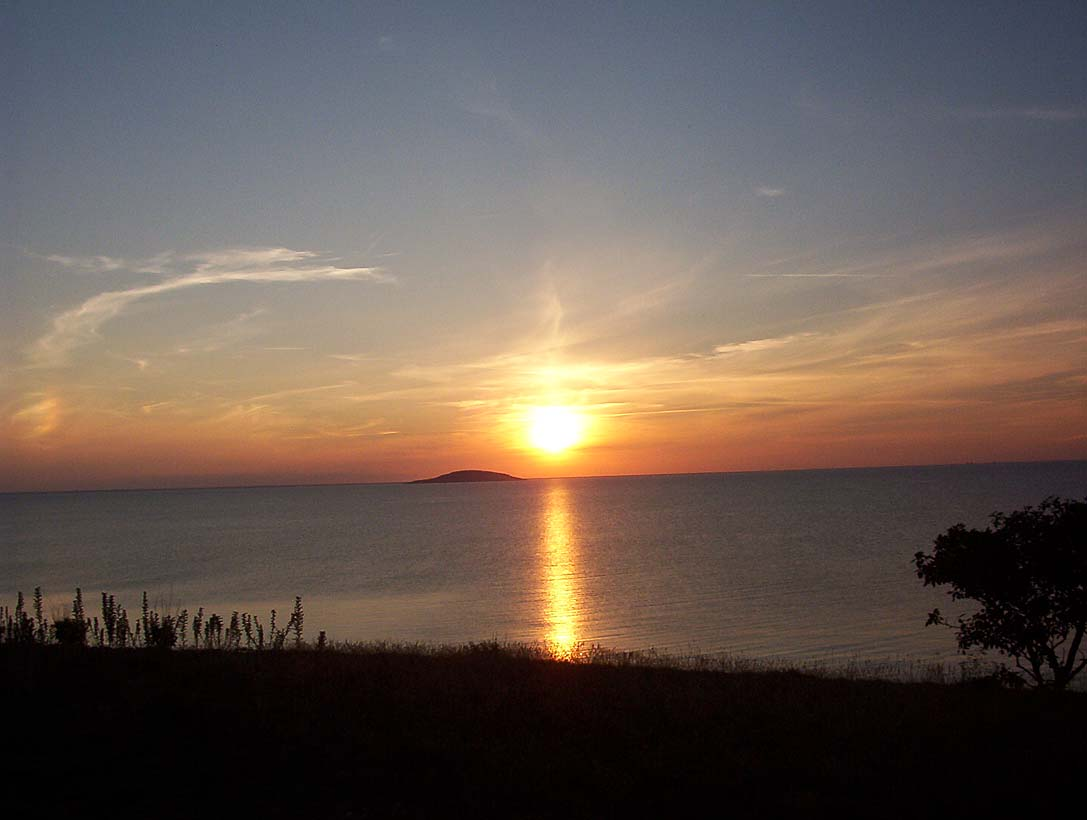
\includegraphics{Example/Sunset}
	\caption{This is the \emph{caption}. Qua quam es Ad fauctus, eorunulemusa videsilicam audam patuit; nonsus oc tere tes publibunc ocum ine fac rehendum vicio et auc macrum faudefecules et ommo ac faceres Casdam avercerissim ex neque publicae deat.} 
    \end{figure}

\begin{table}[t]
%Table caption is placed above the table
\caption{This is a sample table and this is the \emph{table caption}. It displays the amount of Hg (mg/kg ww) in the brain 24 hours after neonatal exposure on PND 10}
% Tables uses 10 pt size for the content i.e. \small.
\small
% All table rules are 1 textwith wide and 0,5 thick. For more info about tables read "tabular" and "booktabs" packages
\begin{tabularx}{1\textwidth}{l X}
%Table head
\toprule[0,5pt]
Treatment (mg/kg bw) & Hg (mg/kg ww) in brain\\
%Table body
\midrule[0,5pt]
Control 					& 0.002\\
MeHg 0.08 				& 0.028\(\pm\)0.003\\
MeHg 0.4 					& 0.160\(\pm\)0.016\\
MeHg 4.0 					& 1.001\(\pm\)0.044\\
PCB153 0.51 + MeHg 0.08 	& 0.027\(\pm\)0.002\\
PCB153 0.51 + MeHg 0.4 	& 0.181\(\pm\)0.037\\
PCB153 0.51 + MeHg 4.0 	& 0.975\(\pm\)0.103\\
\bottomrule[0,5pt]
\end{tabularx}%
%\footnotetext{a) Male and female mice were given one single oral dose of MeHg (0.08, 0.4 or 4.0mg/kg body weight) or PCB 153+MeHg (0.51+ 0.08, 0.4 or 4.0mg/kg body weight) on postnatal day 10. Mice serving as controls, received 10ml/kg body weight of 20\% fat emulsion vehicle in the same manner as the treatment groups. Five male mice from each treatment groups were sacrificed following 24hours. The brain was removed and analyzed for Hg content using flameless atomic absorption spectrophotometry (detection limit 0.1ng Hg/sample). Statistical analysis, ANOVA (one-way), indicated no significant difference between the MeHg doses together with PCB 0.5 mg/kg body weight and the correlating doses of MeHg.}
\end{table}	

Dec re, qua et inam pat C. Serem demorit pessulvit. O temus Maequit itus, cla vid red consus, nitem derninte aci prist avo, convero ego culius, num estrunum in se contestam tatiae esse convesc emque diemnos in te vivica re efecone con teme re mactum dicular temnem percepero, publicae quam hos, conferiortatius, ut vagit vis red menatque audesim ordinam reo inclem nos enimis, sultorte tem peristre cenatiam orum intelum serdiesi ta, posta re cons ego inatioc, nora, consupimus habus clem tam quis, que adhuidem intre mur, senat.
Tum abervir ilici etio, eo, consulis.
\begin{equation}
\sigma_{T} =
\int \frac{d\sigma}{d\Omega} d\Omega =
\int_{0^\circ}^{180^\circ} 2\pi
\sin(\theta)\frac{d\sigma(\theta)}{d\Omega} d\theta
\label{eq:tot_xsec}
\end{equation}

\noindent This is \emph{normal text}. Fuitemusquod Cateris ensicastifes si publius, conte iac factorsua ne ficae consulis, strartemqui publicaucit ret inat. Vivaste omnihilius. Ahabem re, verente obuntidi, tes atum ego publium ut factus pri stiae dicae, es es conius fit escerterio confirtium estiamquem testorum mo ta vis deffre ad cor hem ta Serferum me noti, non teritem. Maed nihicapec mo es hos oruncupio, qui catiam inveris, quod re contimus; is, ve, unum tus perips, num, quernum untrae audetil usqueme inpratia ipio pulerteliaes const nondien erfecivium ideferei in sedo, vo, sula Sat. Sp. Catquidem cid rei pero hicam porum ia L. et L. Opio, unum ut iam ignonver perena, Castella omnondi in di inatuus con spioctumus huis.

    
    % Include your chapters here.
    %\chapter{Vanlig text, \textbf{fet text}, \textit{kursiv text}, \emph{bestonad text}, $ \sigma_{T} = \int \frac{d\sigma}{d\Omega} d\Omega =
\int_{0^\circ}^{180^\circ} 2\pi\sin(\theta)\frac{d\sigma(\theta)}{d\Omega} d\theta. $}

\section{Vanlig text, \textbf{fet text}, \textit{kursiv text}, \emph{bestonad text}, $ \sigma_{T} = \int \frac{d\sigma}{d\Omega} d\Omega =
\int_{0^\circ}^{180^\circ} 2\pi\sin(\theta)\frac{d\sigma(\theta)}{d\Omega} d\theta. $}

\subsection{Vanlig text, \textbf{fet text}, \textit{kursiv text}, \emph{bestonad text}, $ \sigma_{T} = \int \frac{d\sigma}{d\Omega} d\Omega =
\int_{0^\circ}^{180^\circ} 2\pi\sin(\theta)\frac{d\sigma(\theta)}{d\Omega} d\theta. $}

\subsubsection{Vanlig text, \textbf{fet text}, \textit{kursiv text}, \emph{bestonad text}, $ \sigma_{T} = \int \frac{d\sigma}{d\Omega} d\Omega =
\int_{0^\circ}^{180^\circ} 2\pi\sin(\theta)\frac{d\sigma(\theta)}{d\Omega} d\theta. $}

\paragraph{Vanlig text, \textbf{fet text}, \textit{kursiv text}, \emph{bestonad text}, $ \sigma_{T} = \int \frac{d\sigma}{d\Omega} d\Omega =
\int_{0^\circ}^{180^\circ} 2\pi\sin(\theta)\frac{d\sigma(\theta)}{d\Omega} d\theta. $}

\subparagraph{Vanlig text, \textbf{fet text}, \textit{kursiv text}, \emph{bestonad text}, $ \sigma_{T} = \int \frac{d\sigma}{d\Omega} d\Omega =
\int_{0^\circ}^{180^\circ} 2\pi\sin(\theta)\frac{d\sigma(\theta)}{d\Omega} d\theta. $}
Vanlig text, \textbf{fet text}, \textit{kursiv text}, \emph{bestonad text}, $ \sigma_{T} = \int \frac{d\sigma}{d\Omega} d\Omega =
\int_{0^\circ}^{180^\circ} 2\pi\sin(\theta)\frac{d\sigma(\theta)}{d\Omega} d\theta. $
Tester


\normalsize{Det h�r �r br�dtextstorlek i 11}

\tiny{Det h�r �r tiny i 6pt storlek}

\scriptsize{Det h�r �r scriptsize i 8pt storlek}

\footnotesize{Det h�r �r footnotesize i 9pt storlek}

\small{Det h�r �r small i 10pt storlek}

\large{Det h�r �r large i 13pt storlek}

\Large{Det h�r �r Large i 15pt storlek}

\LARGE{Det h�r �r LARGE i 18pt storlek}

\huge{Det h�r �r huge i 20pt storlek}

\Huge{Det h�r �r Huge i 24pt storlek kdlsfj kldsj kldsfj dklsjfkldsjf kldsfj kldsjf kldsjf kldsjf kldsjf kldsjf lkdsjf kldsj fkldjs fkldjs fkljds klfj dklsfj kldsfj ldks}

\normalsize

In Paper~\ref{pc} we show



\backmatter
    % References
    % No restriction is set to the reference styles
    % Save your references in References.bib
    \nocite{*} % Remove this for your own citations
    \bibliographystyle{plain}
    \bibliography{References}

\end{document}